\documentclass{report}
\usepackage[left=3cm,top=2cm,right=3cm]{geometry}

\usepackage{times}
\usepackage[siunitx]{circuitikz}
%\usetikzlibrary{trees}
%\usetikzlibrary{shapes,snakes}
\usepackage{verbatim}
\usepackage{amsmath}
\usepackage{amssymb}
\usepackage{algorithmic}
\usepackage{setspace}
\usepackage{graphicx}
\usepackage{cancel}
\usepackage[colorlinks=true]{hyperref}

\doublespacing

\newcommand{\R}{\mathbb{R}}
\newcommand{\Q}{\mathbb{Q}}
\newcommand{\N}{\mathbb{N}}
\newcommand{\Z}{\mathbb{Z}}
\newcommand{\qed}{\\$\Box$}
\newcommand{\qle}{\stackrel{?}{\le}}
\newcommand{\qeq}{\stackrel{?}{=}}
\newcommand{\closure}{\overline}
\newcommand{\intersect}{\cap}
\newcommand{\union}{\cup}
\newcommand{\nullset}{\emptyset}
\newcommand{\minus}{\ \backslash\ }


\begin{comment}

:Author: Micah Chambers
\end{comment}

\begin{document}
\chapter{Introduction}
Functional Magnetic Resonance Imaging (FMRI) is a powerful tool in the analysis
of neural activity. Despite its rather limited temporal resolution, FMRI is still
the best way of measuring neural activity for the majority of the brain.
Whereas other methods
of analyzing neural signals can be invasive or difficult to acquire, 
FMRI is relatively quick and cheap, and its analysis straight forward.
Because of these benefits, FMRI continues to be crucial to the study of human 
cognition. Despite its prevalence, there have been relatively few developments
in the actual analysis of FMRI images. A steady stream of studies have built
on the original BOLD signal derivation first described in \cite{Ogawa}, 
from the Baloon model first proposed by \cite{Buxton1998}
all the way to full fully autonomous system of equations \cite{Riera2004}. And while
there have been numerous forks in the model, enough in fact to make an entire paper
studying the differences,\cite{Deneux2006}, it is widely known that all these
models have quantitatively less bias error than General Linear Model which is
typically employed today. Then again, depending on the model there may be between
seven \cite{Riera2004} and 50 \cite{Behzadi2005} parameters per voxel to
be optimized. Clearly there is a significant risk of error due to variance
with so many degrees of freedom, not to mention a significantly increased
computation cost. In this thesis I demonstrate the use of a 
particle filter as a means of addressing these problems.

FMRI images as a method of detecting neural activation is based on 
temporal changes of the Blood Oxygen Level Dependent (BOLD) signal.
The BOLD signal is caused by minute changes in the ratio of Deoxygenated
Hemoglobin to Oxygenated Hemoglobin in blood vessels throughout the brain.
Because Deoxygenated hemoglobin is paramagnetic, higher concentrations
attenuate the signal when using T2 weighted imaging techniques, such 
as Echo Planar Imaging (EPI) which is used in FMRI. When axons becomes active,
a large amount of ions quickly flow out of the cell. In order for the action
potential to be used again, an active pumping process moves ions back into the
axon. This process of recharging the axon takes a large amout of enengy, which 
naturally uses oxygen. On a massive scale (cubic millimiter) this activation/recharge
process is happening all
the time; however, it happens at a much higher rate when a portion of
the brain is very active. Thus, blood vessels in a very active area will 
tend to have less oxygenated hemoglobin, and more deoxygenated hemoglobin,
resulting in lower FMRI signal. However, to compensate for activation, muscles that
control blood vessels relax in that region to allow more blow flow, which 
in fact results in a higher concentration of oxygenated hemoglobin. Thus,
increased activation actually tends to \emph{increase} the MR signal in
comparison with the base level. It is this overcompensation that is the 
primary signal detected with FMRI imaging. This cascade of events
can, as a consequence of increased activity, increase the local metabolism, 
blood flow, blood volume, and oxygenated hemoglobin; though not necessarily
in sync. The lag between these
various factors is what causes many of the complexities of the BOLD signal.

\section{FMRI}
Magnetic Resonance Imaging, MRI is a method of building 3D images
non-invasively, based on the difference between nuclear spin
relaxation times in various molecules. Initially the entity being
imaged is brought into a large magnetic field which aligns the spins
of molecules in the same direction; radio frequency (RF) signals may
then be used to excite nuclear spin away from the steady alignment. 
As the nuclei precess back to their original orientation, they resonate
at the same RF frequency of their original excitation. Conveniently, the
excitation of nuclear spins return their original state at different
rates, called the T1 relaxation time, depending on the properties of 
the material excited. Additionally, the
coherence of the spins also decay differently (and quite a bit faster
than T1) based on the properties of the region that has been excited.
This gives two primary methods of contrasting substances,
which is the basis of T1 and T2 weighted images. Additionally, there
dephasing occurs at two different rates, the T2 relaxation time,
which is impossible to recover from, and T2$^*$ relaxation, which is
much faster, but possible to recover from with an inversion pulse.
Oftentimes T1 relaxation times can be on the order of seconds if 
a significant excitation pulse is applied. 
In order to rapidly acquire entire brain images, as is done in Functional 
MRI, a single large excitation pulse is applied to the entire brain,
and the entire volume is acquired in a single T1 relaxation period. 
Because the entire k-space (spatial-frequency) volume is acquired 
from a single excitation, the signal to noise ration is very low
in this type  of imaging (Echo Planar Imaging). 

Increasing the spatial resolution of EPI imaging necessarily 
requires more time or faster magnetic field switching. Increasing
magnet switching rates though is difficult, because it can result in
more artifacts, or even lower signal to noise ratios. The result is
that at \emph{best} FMRI is capable of 1 second temporal resolution. 
Additionally, the means that each voxel of the image will contain 
the sum of a large amount neurons, capillaries and veins. Thus, the
FMRI signal, which is sensitive to the chemical composition of 
materials, is summing up the composition of various types of tissue
in addition to the blood, whose composition is what we actually care about.
In particular, the presence of Deoxyhemoglobin, Hemoglobin whose
oxygen has been used by a metabolic process, has a decreased magnetic
response compared to Oxygenated Hemoglobin. Thus, capillaries near
very active cells will typically have a higher Deoxyhemoglobin content and
lower signal, and regions with lower activity will have a lower 
Deoxyhamoglobin content and thus higher signal.
Unfortunately, as mentioned previously, blood is only a small part of
each voxel, which means that a single EPI image doesn't tell much about
Deoxyhemoglobin content. However assuming blood is the only thing changing
in the short term, percent difference from a baseline signal \emph{will}
tell us something. FMRI analysis is thus necessarily performed on the percent change
from the baseline. Luckily the assumption that tissue content does not change in
the short run is actually pretty good, although other factors can pollute
the baseline signal, as we will discuss later. 

\section{BOLD Physiology}
\label{sec:BOLD Physiology}
It is well known that the two types of hemoglobin act as a contrast agents in 
EPI imaging
\cite{Buxton1998}, \cite{WEISSKOFF1994}, \cite{Ogawa}, however the connection
between Deoxyhemoglobin/Oxygenated Hemoglobin and neural activity is non-trivial. 
Intuitively, increased 
metabolism will increase Deoxyhemoglobin, however blood vessels are quick
to compensate by increasing local blood flow. Increased inflow will of course
preceed increased outflow, and increased inflow is accomplished by loosening 
capilary beds. Both of these factors drive increased storage capacity.
Since the local MR signal depends on the ratio of Deoxyhemoglobin to Oxygenated
Hemoglobin, increased volume of blood can certainly effect this ratio if 
metabolism doesn't exactly match the increased inflow of oxygenated blood.
This was the impetus
for the ground breaking balloon model (\cite{Buxton1998}) and windkessel
model (\cite{Mandeville1999}). These models derive from first principals
the increased deoxyhemoglobin ratio and volume of capillaries based on a given flow.
These were the first two attempts to quantitatively account for the shape of the 
BOLD signal as a consequence of the lag between the cerebral blood volume (CBV) 
and the cerebral blood flow (CBF). In fact \cite{Buxton1998} went to far as
to show that a simple, well chosen blood flow waveform coupled with a square 
wave cerebral metabolic rate of oxygen (CMRO2) curve, in the context of a balloon 
model, could fully account for the BOLD signal. 

Although \cite{Buxton1998} showed that a well chosen flow waveform could 
explain much of the BOLD signal, there was still a matter of proposing a
realistic waveform for the CBF and for the CMRO2. \cite{Friston2000} gave
a reasonable and simple
expressoin for CBF input,$f$, based on a flow inducing signal, $s$, 
\begin{eqnarray}
\dot{s} &=& \epsilon u(t) - \frac{s}{\tau_s} - \frac{f - 1}{\tau_f} \\
\dot{f} &=& s
\end{eqnarray}
where $\epsilon$ is a neuronal efficiency term, $u(t)$ is a stimulus, and $\tau_f$, $\tau_s$
are both time constants. In \cite{Buxton2004} the final piece of the simple balloon
model was put into place, by describing the CMRO2 as a constant multiple of
the CBF (the inflow of blood). This completed the basic balloon model, and 
was well summarized in \cite{Riera2004}. 
\begin{eqnarray}
\dot{v} &=& \frac{1}{\tau_0}(f - v^\alpha)\\
\dot{q} &=& \frac{1}{\tau_0}(\frac{f(1-(1-E_0)^f)}{E_0} - \frac{q}{v^{1-1/\alpha}})
\end{eqnarray}
where $v$ is normalized cerebral blood volume (CBV), and $q$ is the normalized
local deoxyhemoglobin/oxygenated hemoglobin ratio, $E_0$ is the resting metabolic
rate and $\alpha$ is Grubb's parameter controling the balloon model. 
\cite{Obata2004} refined the readout equation of the BOLD signal based on the
deoxyhemoglobin content (q) and local blood volume (v), resulting in the
final BOLD equation:
\begin{eqnarray}
y   &=& V_0((k_1 + k_2)(1-q) - (k_2 + k_3)(1-v))\\
k_1 &=& 4.3 \times \nu_0 \times E_0 \times TE = 2.8\\
K_2 &=& \epsilon_0 \times r_0 \times E_0 \times TE = .57\\
k_3 &=& \epsilon_0 - 1 = .43
\end{eqnarray}
Where $\nu_0 = 40.3 s^{-1}$  is the frequency offset in Hz for fully
deoxygenated blood (at 1.5T), $r_0 = 25 s^{-1}$  is the slope relating
change in relaxation rate with change in blood oxygenation, and
$\epsilon_0 = 1.43$ is the 
ratio of signal MR from intravascular to extravascular at rest. Although,
obviously these constants change with experiment ($TE$, $\nu_0$, $r_0$),
patient, and brain 
region ($E_0$, $r_0$), often the estimated values taken from \cite{Obata2004} are used
as constants ($k_1 + k_2 = 3.4$, and $k_2+k_3 = 1$) in 1.5 Tesla studies..
While this model is in a sense complete, it is far from perfect. The major
problem often brought up with this version of the BOLD model is that it
does not represent the so called "post-stimulus undershoot" well.
The post-stimulus undershoot is the name for a prolonged sub-normal
BOLD response for a period of 10 to 60 seconds after stimulus has
ceased (\cite{Chen2009}, \cite{Mandeville1999a}).

There are two theories for the cause of the post stimulus undershoot. Recall
that a lower than base signal means that there is an increased deoxyhemoglobin
content in the voxel. The first and simplest explanation is that the post-stimulus
undershoot is caused by a prolonged increase in CMRO2 after CBV and CBF
have returned to their base levels. This theory is justified by quite a few
studies that show CBV and CBF returning to the baseline before the BOLD signal
(\cite{Frahm2008}, \cite{Donahue2009}, \cite{Buxton2004}, \cite{Lu2004},
\cite{Shen2008}). Unfortunately, because of limitations on FMRI and en vivo
CBV/CBF measurement techniques it is difficult to isolate whether CBF and
CBV truly have returned to their baseline. Other research seems to indicate
that there can be a prolonged residual supernormal CBV (\cite{Mandeville1999a}, 
\cite{Behzadi2005}, \cite{Chen2009a}), although none of these papers completely
rule out the possiblity of increased CMRO2. Additionally, in \cite{Yacoub2006}, it 
was found that the post-stimulus undershoot varried across regions of the brain, 
which could further explain the contradictions found elsewhere. \cite{Chen2009a}
makes a compelling case that most of the post stimulus undershoot could be 
explained be a prolonged CBV increase, and a prolonged CBF undershoot, and that
many of the previous measurements showing a quick recovery of CBV 
may have been dominated arterial CBV's return to baseline. 

Because of the significant possility of a completely independent CMRO2,
extremely complex models for metabolism exist (\cite{Zheng2005}), although 
most recent studies have
focused on their ability to explain the prolonged BOLD post stimulus 
undershoot \cite{Zheng2005}, \cite{Buxton2004}. This is because \cite{Buxton2004}
and later \cite{Riera2004} showed that the main portion of the signal may be 
accurately estimated by a simple blood flow locked expression of the CMRO2.. 
Although \cite{Deneux2006} did not deal extensively with prolonged post
stimulus undershoot, the comparisons made in that publication showed minimal
improvement from separate expressions of CMRO2, in comparison to the much 
increased complexity. \cite{Deneux2006} did show that by simply adding viscoelastic
terms, first proposed in \cite{Buxton2004}, that a slowed return to baseline for
the BOLD signal is possible to model. However, viscoelastic effects primarily
control CBV, which, as mentioned already, many studies have claimed cannot be 
responsible for the BOLD post-stimulus undershoot. Another extensive model
that attempts to quantify the post-stimulus undershoot is the compliance model 
proposed by \cite{Behzadi2005}. Although through a somewhat different means than
the \cite{Zheng2005} and \cite{Buxton2004} papers, its possible the increased
model flexibility ultimately is the key reason for the improvements, as opposed
to increased plausibility. Because of these controversies, and because this is
the first time a particle filter has been used for this problem in this way, 
our aim to keep the model simple was best met by using the original balloon
model with the possible addition of the visco-elastic effects from \cite{Buxton2004}.

Even more advanced versions of the Balloon model exist. In fact \cite{Buxton2004}
introduced several additional state variables, including the CMRO2, the O2 extraction
fraction, which is closely related to CMR02, and the neural response, which 
causes the stimulus to decay toward some steady state value. The 
neural response is intended to emulate neural habituation, wherein neurons
become less sensitive to a prolonged stimulus. While these advanced may be more
capable of capturing a more exact version of the BOLD signal, the difference
between the model will often times be below the noise floor. In essence this 
is a classic bias-variance
dilemma: at some point increased model flexibility, and thus variance, is not
worth the decrease in model bias. For now it remains to be seen where this
line may be drawn in the BOLD signal, although \cite{Deneux2006} does not
show a significant improvement from the additional parameters added in 
\cite{Buxton2004}.

\section{Previous Studies of Parameters}
There have been quite a few efforts to quantify the parameters of the
various BOLD models.  Although \cite{Buxton1998} and \cite{Friston2000}
both proposed physiologically reasonable values for the model parameters, 
\cite{Friston2002} was the first paper to calculate the parameters based 
on actual FMRI data. In that paper, Friston et. al. used a variation of
Expectation Maximization to find a normal distribution for the parameters:
\begin{eqnarray}
\epsilon &=& N(.54 , .1 ^2 )  \nonumber \\
\tau_s & =&  N(1.54, .25^2)   \nonumber \\
\tau_f & =&  N(2.46, .25^2)   \nonumber \\
\tau_0 & =&  N(.98 , .25^2 )   \nonumber \\
\alpha & =&  N(.33 , .45^2 )   \nonumber \\
E_0   & =&  N(.34 ,  .1 ^2 )   \nonumber \\
V_0  & = &  .03 (not\ estimated) \nonumber
\end{eqnarray}
Since then, several other methods of have been used to calculate
BOLD parameters from FMRI timecourses. In \cite{Riera2004}, a maximum
likelihood method for innovation processes was used, as described by
\cite{Ozaki1994}. \cite{Ozaki1994} uses a similar construction to a 
Kalman filter, to break the time series into a series of innovations,
for which Maximum Likelihood was performed. While this is in some since the
"right" way to find the solution, it comes with several caveats. First, every
step in parameter space requires a recalculation of all the state variables. With
two or three parameters this is fine, more than that, and calculations could go on
indefinitely. Second, it still assumes the parameters and noise are Gaussian, and
will only be optimal in that case. Third, depending on the nonlinearities present
in the system, local minima may be extremely common. Later \cite{Hu2009} used an 
Unscented Kalman Filter over all the parameters and state variables to find the 
parameter set/variable time series. While this method has the drawback of not necessarily
being optimal, unfortunately there is no general optimal solution to non-linear non
Gaussian models. Hu et. al.'s technique also will run significantly faster than
ML based techniques, since it does not require recalculating the entire timeseries
for every step in parameters. Both \cite{Hu2009} and \cite{Friston2002} came to results 
very similar to the expected values stated in \cite{Buxton1998} and \cite{Friston2000}.
One potential problem with all these techniques are that the depend heavily on the
priors. The starting point of the parameters could have a huge impact on the
results, and while one can be hopeful that this isn't the reason for the agreement
between \cite{Friston2000} and later results, there is no way to know. 

In \cite{Johnston2008}, a hybrid particle filter/gradient
descent algorithm was used to simultaneously derive the static (classicly called
parameters) and dynamic parameters (classically known as state variables).
Essentially a particle filter is used to calculate the state variables at some
time, and then the estimated distribution of the particles was used to find
the most likely set of parameters that would give that distribution of state variables.
\cite{Johnston2008} comes to a very different set of parameter estimates as compared
to the original \cite{Friston2000} guesses:
\begin{eqnarray}
epsilon &=& .069 \pm .014    \nonumber \\
tau_s & =& 4.98 \pm 1.07  \nonumber \\
tau_f & =& 8.31 \pm 1.51   \nonumber \\
tau_0 & =& 8.38 \pm 1.5    \nonumber \\
alpha & =& .189 \pm .004   \nonumber \\
E_0   & =& .635 \pm .072     \nonumber \\
V_0   & =& .0149 \pm .006     \nonumber 
\end{eqnarray}
Notably, the time constants are significantly longer. This could be a result of
some preprocessing to the stimulus timeseries performed in \cite{Friston2002} and
later works but not in \cite{Johnston2008}, or it could be that \cite{Johnston2008}
depended less on the priors. 

Its possible, although unlikely that the balloon model is not possible to learn
without detrimental cost in variance error. I do not think this is the case, however,
and I will work to dispell this possibility in the results with simulated time
series.

\section{Noise}
Thus, despite some discrepencies, the cause of the BOLD signal is
relatively well known.  but FMRI doesn't detect this happening in one neuron,
but rather as the 
aggregate over millions of cells. Though local neurons act
"together" (i.e. around the same time), the density of neurons, the
density of capillaries, and slight differences in activation across 
a particular voxel can all lead to signal attenuation or noise. 
A particularly insidious type of noise present in FMRI is a low frequncey
drift, first characterized by a Weiner process in \cite{Riera2004}. 
Though not present in all regions, it is prevalent enough to cause significant
inference problems \cite{Tanabe2002}. It is still not
clear where exactly this noise comes from, although it is possible it is 
the result of magnets heating up, or some distortion in magnetic
fields \cite{Smith2007}. It is clear that this drift signal is not soley
due to a physiological
effects, given its presence in cadavers and phantoms \cite{Smith1999}.
Additionally, since it is standard operating procedure to perform
co-registration between volumes, it is unlikely that movement was
the cause of the drift either (otherwise the effect would not be 
widely reported).

In order to characterize the noise in the FMRI we took a few 
sample time-series during resting state, which should theoretically be all noise and 
used Q-Q plots to analyze the type of noise present. Additionally, the autocorrelation
was also calculated since most methods (including the one used in this paper)
assume the noise is independent from time and
identically distributed.  If these assumptions fail, then error rate will
be higher than expected. \autoref{fig:QQDC} shows the 
results with a regression line fit to the points. A set of points that are exactly 
Gaussian should all fall on the same line.  Because it the noise is often considered 
to have Weiner noise with Gaussian steps, as first described in \cite{Riera2003}, we
also performed the same tests again, but on the steps, rather than the 
direct measurements. \autoref{fig:QQDelta} shows the analysis of the same
set of time-series as \autoref{fig:QQDC}, after being converted to steps.
Finally, as we will discuss in \autoref{sec:Methods Preprocessing}, some
amount of drift can be removed by subtracting off a spline from the timeseries.

\begin{figure}
\caption{Q-Q Plots of resting state data}
\label{fig:QQDC}
\end{figure}

\begin{figure}
\caption{Q-Q Plots of resting state data, using the steps as the samples}
\label{fig:QQDelta}
\end{figure}

<conclusion about the noise>

\section{Analysis of the BOLD Signal}
Several studies have endeavored to analyze the BOLD equations, which
we will review here. The most obvious analysis is to calculate the
steady state signal, when $u$ is held constant long enough for
all the transients to settle out. 

\begin{eqnarray}
s_{ss} &=& 0 \nonumber \\
f_{ss} &=& \tau_f\epsilon u + 1\nonumber \\
v_{ss} &=& (\tau_f\epsilon u + 1)^\alpha\nonumber \\
q_{ss} &=& \frac{(\tau_f\epsilon u + 1)^\alpha}{E_0}(1-(1-E_0)^{1/(\tau_f\epsilon u + 1)})\nonumber \\
y_{ss} &=& V_0((k_1+k_2)(1-q_{ss}) - (k_2+k_3)(1-v_{ss}))
\label{eq:steadystate}
\end{eqnarray}

[Image with two different $\alpha$'s]

[image comparing the results of 10\% changes in various signals]


\chapter{Current Techniques}
\section{Basic Statistical Parametric Mapping}
Although not strictly the same thing as parameter calculation from 
FMRI, activation detection is very similar. In fact, estimation of 
parameters is somewhat a generalization of the idea of activation detection.
Thus, it is important to draw a comparison between the methods proposed
in this thesis with existing methods of activation detection.

The most basic method of analyzing FMRI data is through a standard T-test
between "resting state" and "active state" samples. This is done by 
taking the average and variance of the inactive period, and the 
period during which the stimulus was activate separately then treating 
them both as gaussian distributions.
If they are in fact Gaussian distributions, then a basic t-test will
give the probability that the samples came from the same distribution
(the null hypothesis). Of course, this test is fraught with problems; even if
the drift mentioned earlier has been removed, there is little reason
to believe that the noise is Gaussian, or even stable. Additionally, 
even if the noise were Gaussian, a t-test with a p-value of .05 over
50000 or more samples is on average going to generate $.05*50000$ false
positives. To compensate for this, bonferoni correction, also known as
multiple comparison tests are performed; essentially p-values are 
divided by the number of independent
tests being run. This, however, leads to extremely low p-values, so
low that it would be impossible for any biological system to satisfy. To
compensate, a Gaussian kernel is applied to the image, thus reducing
variance (and thus separating the active and inactive distributions)
as well as decreasing the effective number of voxels. Since t-tests are
now no longer being applied to n <I need to define n> independent voxels,
the factor by which the p-value must be divided by can be decreased.
<Do I need to mathematically define all this?> The derivation and application
of random field theory, and its use can be found in various papers \cite{Worsley2004}.

\section{General Linear Model}
The most used form of FMRI analysis is Statistical Parametric
Mapping, but is able to account for several different levels or types
of stimulus (see \cite{Hofmann1997}). By using hierarchical models
the output signal timeseries is considered the weighted
sum of the various input timeseries. Essentially every experimental factor
is considered as another level inputs (ex. different type of stimulus,
different run with the same patient, different patient). 
The equation for a general linear model is then
\begin{equation}
Y(t) = X(t)\beta + \epsilon(t)
\end{equation}
where $Y(t)$ is the smoothed or detrended timeseries of measurements,
$X(t)$ is a row vector of input, $\beta$ is a column vector of weights,
and $\epsilon$ is the error. Thus for every time, the measurement is
assumed to be a weighted sum of the columns of $X$ plus some error. The calculation
of $\beta$ is then performed using a maximum likelihood or gradient descent search 
to minimize the error.

[Image of GLM]

It is well known of course that a square wave stimulus does not result in a square wave
in the activation of brain regions. Thus, various methods are used to 
smooth the columns of $X$, and thus bandlimit the input. 
The best technique is convolving the stimulus input with a Hemodynamic 
Response Function (HRF), which mimics the basic shape of BOLD activation, including a delay
due to rise time and fall time. The downside of this method, however is that 
the shape of the Hemodynamic Signal is static, meaning the same Hemodynamic Function is
used for every region of the brain, and $Y(t)$ must linear combination 
of scalar the columns of $X$ to be appropriately identified. Additionally, 
it is well known that different Hemodynamic Response Functions are necessary for different 
regions of the brain. The "Canonical" HRF that is most used, has been fitted
for the visual cortex. Thus the shape of the HRF may differ significantly in
terms of onset and fall time in other areas of the brain. The inability to
fit parameters other than scale certainly hinders SPM's
ability to locate voxels that do not conform to the "canonical" hemodynamic 
response function. If there are different HRF's for different regions 
of the brain, might there also be more subtle differences even within
a particular region? It seems reasonable to think so. As a result, the 
most common use of SPM will be heavily biased toward the visual cortex.

[Image of Hemodynamic Response Function]

The GLM is extremely powerful at determining the linear dependence of
a set of regressors on the output. Unfortunately, there is significant evidence
that many of these dependencies are nonlinear, which means they may be
difficult or impossible to detect using linear techniques. This presents
a significant and unknown problem that is often left un-addressed in 
neural studies.

A static linear model is also unable to incorporate other forms of physiological
data that may be available. Combined FMRI
CBF or CBV imaging methods are not uncommon and they could shed much light on
neural activation. However, there is no way of actively combining that data 
into a static HRF. The fact of the matter is that the relation between the 
BOLD signal and CBV/CBF simply cannot be described by any linear relationship.
While it may be possible to determine some regionally varying set of parameters
for the HRF based on CBV/CBF, the lack of physiologically inspired parameters
impairs this. The importance of regional differences in the HRF cannot be
over-stated; it is well known that capillary beds are far from uniformly distributed
and thus blood perfusion and regional oxygenation cannot possibly be uniform
either. 

Finally, all these techniques require the noise to be Gaussian to reach
an optimal solution. In fact there is no known optimal solution to
nonlinear models with non-Guassian noise, so obviously some assumptions
are going to have to be made to reach a solution. However, it would be
nice to have an algorithm that is robust to these effects, and could
still give a good solution when Gaussianity is violated.

Because of these limitations, its entirely possible that activation exists
in regions that SPM doesn't detect, but because the activation does not conform
to the set HRF, it is impossible for these signals to be detected. Perhaps
because of this, it is not uncommon for data to be thrown out or averaged
together in FMRI studies because 
no significant activation could be seen in a single run \cite{Riera2004}
\cite{Johnston2008}. This practice highlights 
limitations in strictly linear approaches; and suggests that a single HRF is 
insufficiently flexible to account for relatively common variations of neural activation. 

In general activation detection type methods also don't have the ability 
to find pathologies based on state variables or parameters.  It
is quite possible that physical properties such as decreased compliance of
blood vessels could indicate a neurological condition that is not easily
seen in a T1 or T2 map. In essence, this could make FMRI a much more 
useful clinical tool than it is now. 

\section{Unscented Kalman Filter}
The unscented kalman filter is a powerful gaussian/bayes filter that attempts
to model the posterior distribution of dynamical systems as a multivariate
Gaussian. The Unscented Kalman Filter (UKF) generalizes the Extended Kalman
Filter by allowing the state update to be a function, $g$,

\begin{eqnarray}
X(t) &=& g(u(t), X(t-1))\\
Y(t) &=& h(X(t)
\end{eqnarray}

In order to estimate the posterior at $t$, a deterministic set of "sigma" points 
(often 2 per dimension, plus 1 at the mode of the multivariate distribution)
weighted according to a Gaussian estimate of $X(t-1)$ are passed through
the update equation. This set of points are then used to estimate the 
mean and covariance of $X(t)$. The benefit of this, is that it requires
no Jacobian and only a few extra calculations to get a decent esimate of
a posterior Gaussian. In the BOLD case, the set of equations we are modeling have no 
closed form solution, and finding the Jacobian is impossible without approximations. Although 
\cite{Riera2004}, \cite{Hu2009} mention a Jacobian of the BOLD response, this is
not strictly the case and is rather $\frac{\partial J}{\partial t}$
rather than a true Jacobian.  This is important because the Extended
Kalman filter depends on the Jacobian to map a Gaussian through the 
advancement of time. Thus the popular Extended Kalman Filter won't work
in this case, whereas the Unscented Kalman Filter still does. In fact
\cite{Hu2009} uses the UKF to perform a similar type of analysis to
the one performed in this work. 

\begin{figure}
\caption{Examples of update distributions, using an Kalman Filter, \cite{Thrun2005}}
\label{fig:EKFWorking}
\end{figure}

The difficulty
of using a Kalman Filter, however, is that it assumes a multivariate 
Gaussian for the state variables, $X(t-1)$. The problem with this is that 
when a system is significantly nonlinear, the state at 
$X(t)$ will almost certainly be non-Gaussian, and thus estimating
$X(t+1)$ with $X(t)$ as a multivariate Gaussian will perpetually introduce
error in the distribution. Furthermore, it is not really known what 
sort of underlying distributions may exist in such a mixed biological,
mechanical, chemical system such as the brain. Assuming the parameters
all to be Gaussian may in fact be a gross error. On the other hand, for
small variances and short time steps the gaussiann distribution is a good 
fit, and so in some limited cases the Unscented Kalman Filter could work
well. These are 
non-trivial issues given that the assumption of Gaussianity is what allows
the UKF to estimate the posterior using only the first and second moments;
two parameters that don't uniquely describe most distributions.

\begin{table}[t]
\centering
\begin{tabular}{|c || c |}
\hline 
Parameter & Run 1 \\
\hline
$\tau_0$ & .98  \\
$\alpha$ & .33 \\
$E_0$ & .34  \\
$V_0$ & .03  \\
$\tau_s$ & 1.54  \\
$\tau_f$ & 2.46  \\
$\epsilon$ & .54  \\
$V_t$ & N(1, .3)  \\
$Q_t$ & N(1, .3)  \\
$S_t$ & N(1, .3) \\
$F_t$ & N(1, .3) \\
\hline
\end{tabular}
\caption{Parameters used to test Gaussianity of variables after being transitioned through
the BOLD model}
\label{tab:steptable} 
\end{table}

To determine the amount of error incurred in a Gaussian estimate during
a typical sample period, the states of BOLD equations were assigned according
to four dimensional Gaussian. The states were then propagated through two
seconds of simulation (a typical TR in FMRI) and then the resulting
marginal distributions were compared with a Gaussian distribution. The 
purpose is to determine the degree to which the results of simulation will
result in non-Gaussian output, given a Gaussian input. This also demonstrates
the degree of nonlinearity present in the system. The parameters used are 
shown in \autoref{tab:steptable}

Notably $s_t$ has intentionally been set to a non-equilibrium, but physiologically
plausible value. The value of $u$ is left at zero the entire time, so the 
system will decay naturally (see \autoref{sec:BOLD Physiology}), though initializing 
$s$ at a non-zero level will drive the system for several seconds. 
\autoref{fig:transp1s} shows the results when the system is essentially
left on for 100 milliseconds after setting the variables according to \autoref{tab:steptable}.
The Q-Q plots fit very will with a Gaussian, demonstrating that at this short
time interval nonlinearities have not yet begun to effect the distribution.
However, \autoref{fig:trans1s} us the result after 1 second, which is faster
than most FMRI scanners are capable of sampling at. At that range the tails 
of the distributions for $v$ and $q$ are clearly starting to deviate from the
Gaussian distribution. As a result the uncertainty in $y$ is deviating from
the Gaussian distribution as well. This is important, because although 
approximating the distribution with a Gaussian based on the first two
moments will work in the short run, there will be residual error in the
distribution. 

On the other hand, this effect is more limited if the initial variance is somewhat
smaller. In tests with those cases, it took much longer for the nonlinearities to skew
the distribution. That result could be encouraging to those looking to use the
UKF, if the distributions are kept relatively thin.

Another potential problem with the UKF is that typically the sigma points,
used to estimate the posterior probability, $P(X(t) | X(t-1), u(t))$, are
located on the main axes. As a result, the covariances are not allowed to 
be effected by the state transition the same way the variances are. While
this may be reasonable in low-dimensional systems, high dimensional systems
have a much greater potential for interplay between the variables. While
this problem is relatively easy to fix (by using more sigma points off
the main axes), there is a definite cost in complexity.

Ultimately, there is a distinct possibility that the nonlinearities of 
the BOLD model make Gaussian estimates unrealistic and thus less effective.
More advanced tests where static variables such as $\alpha$ are varied
as well could shed even more light on the issue. The trouble with using
the UKF then to estimate parameters is that all eleven members of $X$ would
be treated like a single joint Gaussian distribution which certainly 
compound the issues of nonlinearity seen in \autoref{fig:transp1s} and 
\autoref{fig:trans1s}

\begin{figure}
\centering
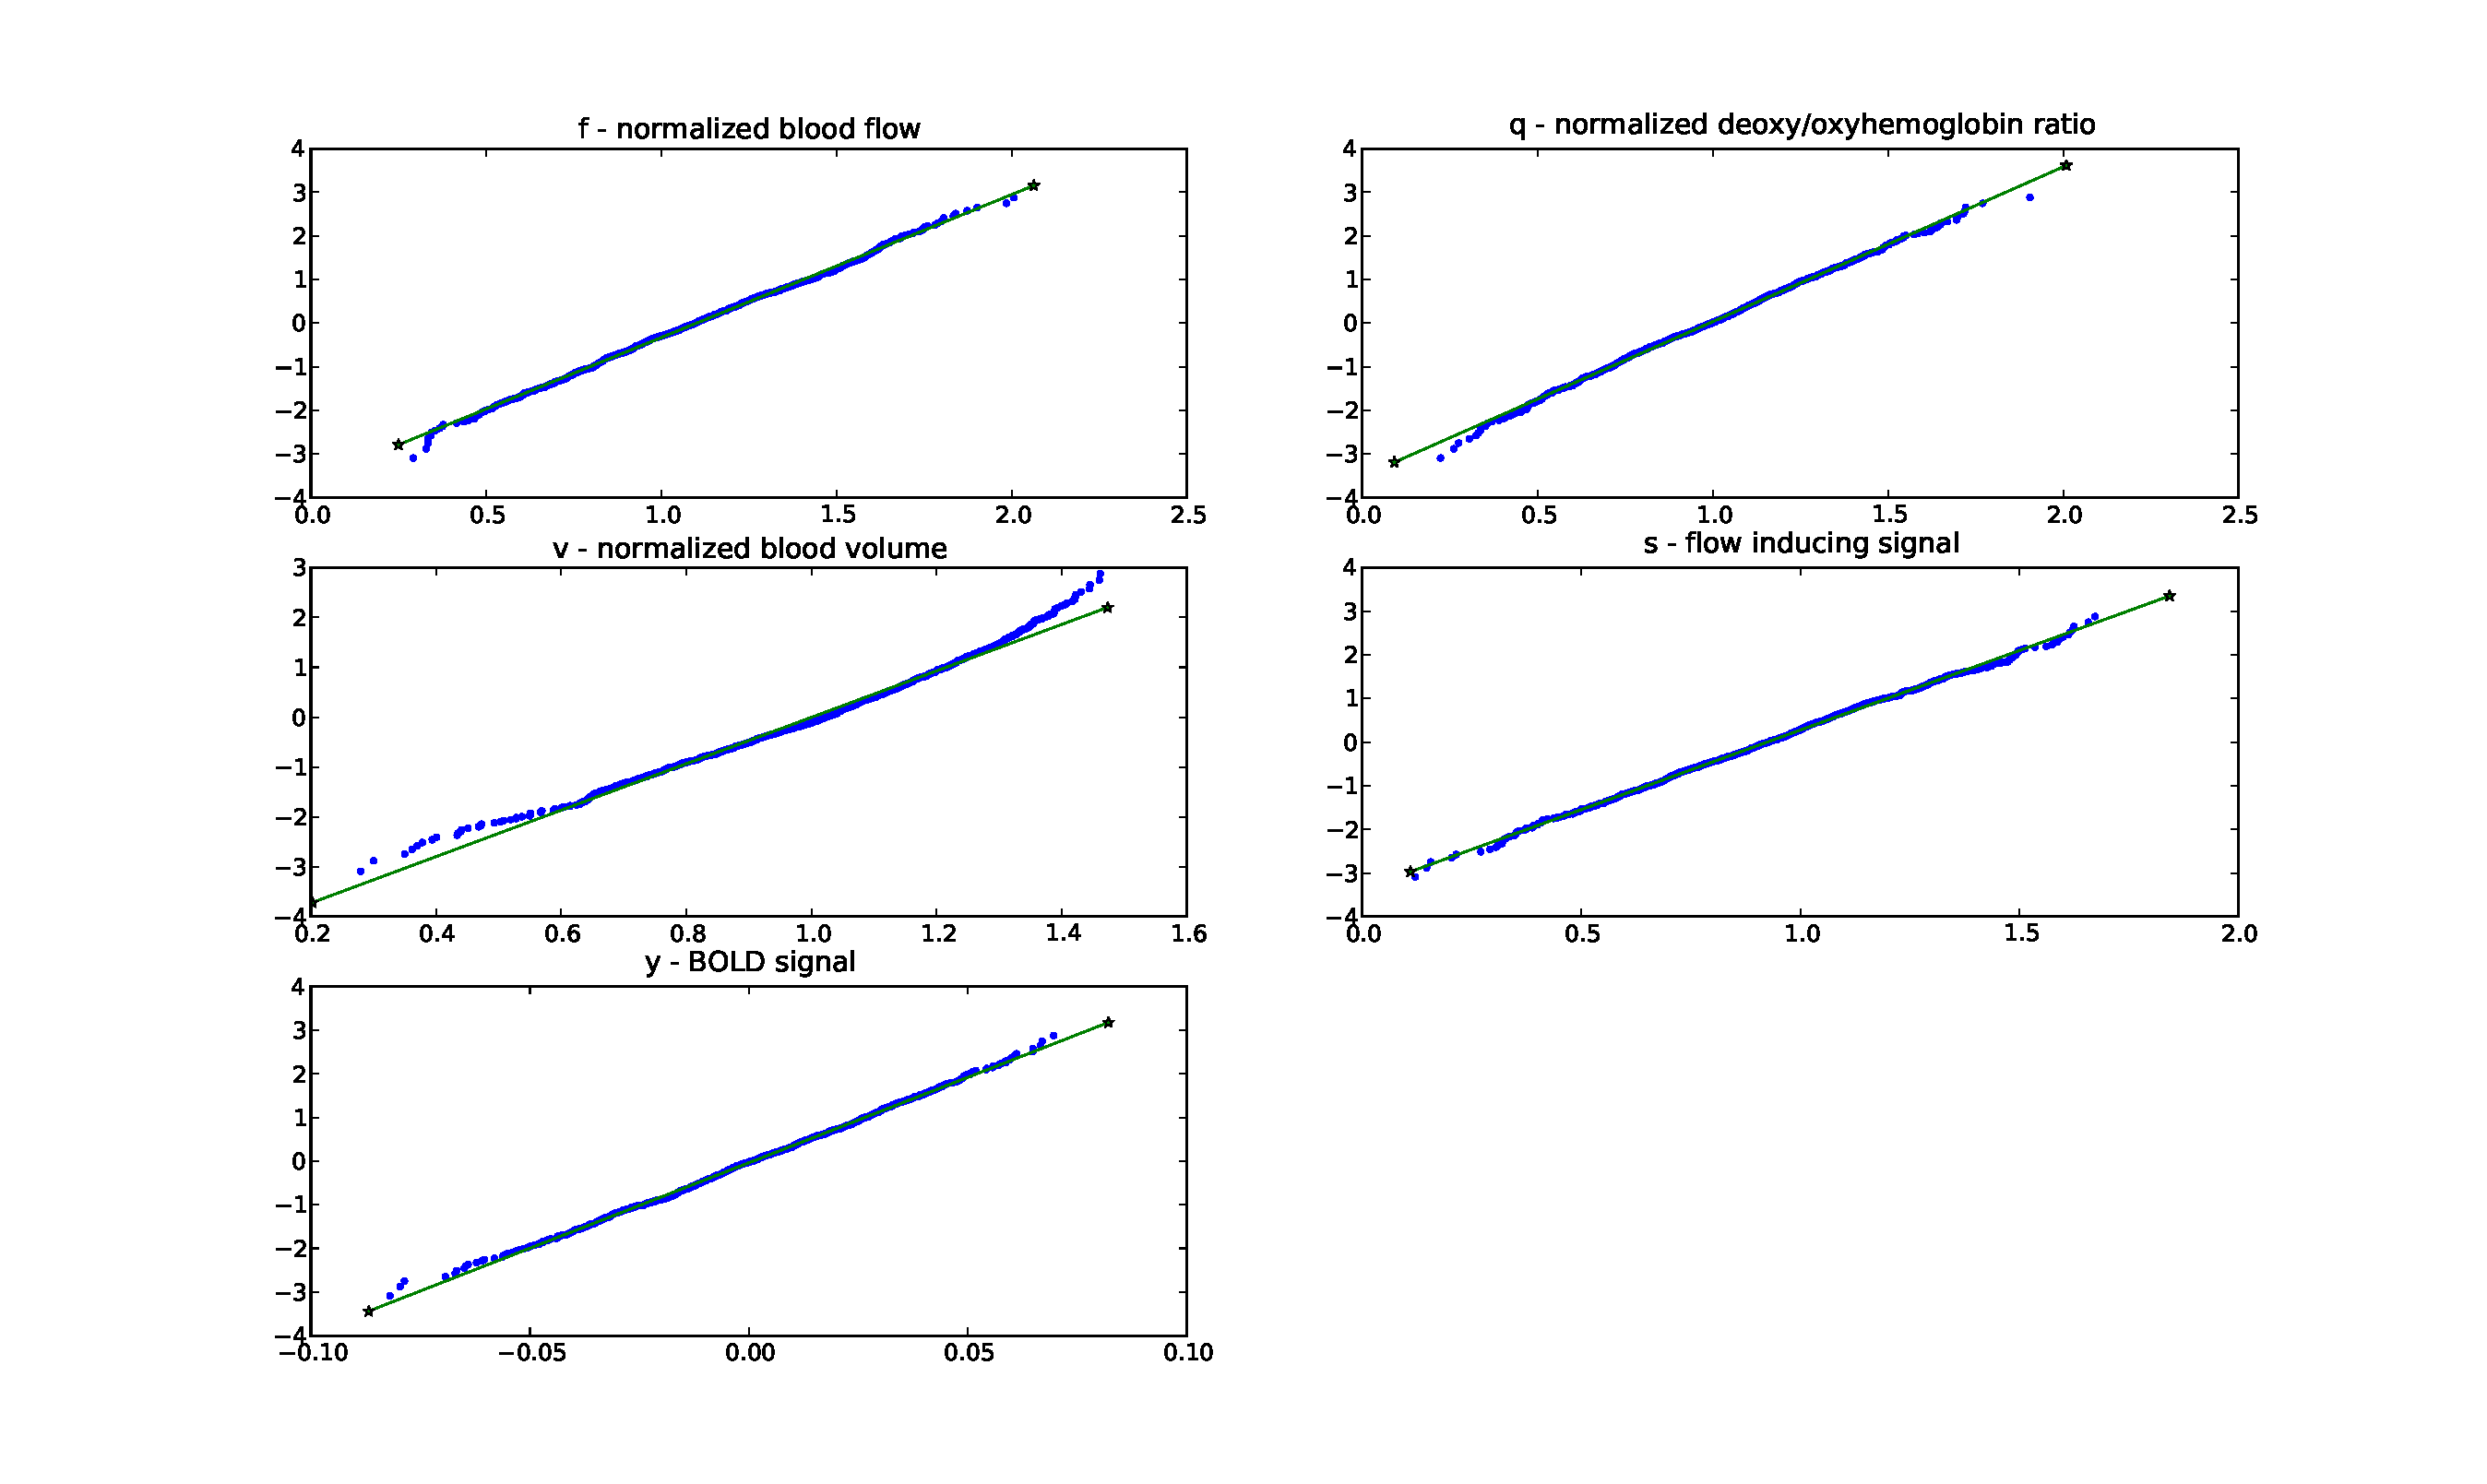
\includegraphics[trim=6cm .75cm 6cm .75cm,width=16cm]{images/gauss_step_point1sec_3sigma.pdf}
\caption{Distributions of state variables after simulating for .1s}
\label{fig:transp1s}
\end{figure}

\begin{figure}
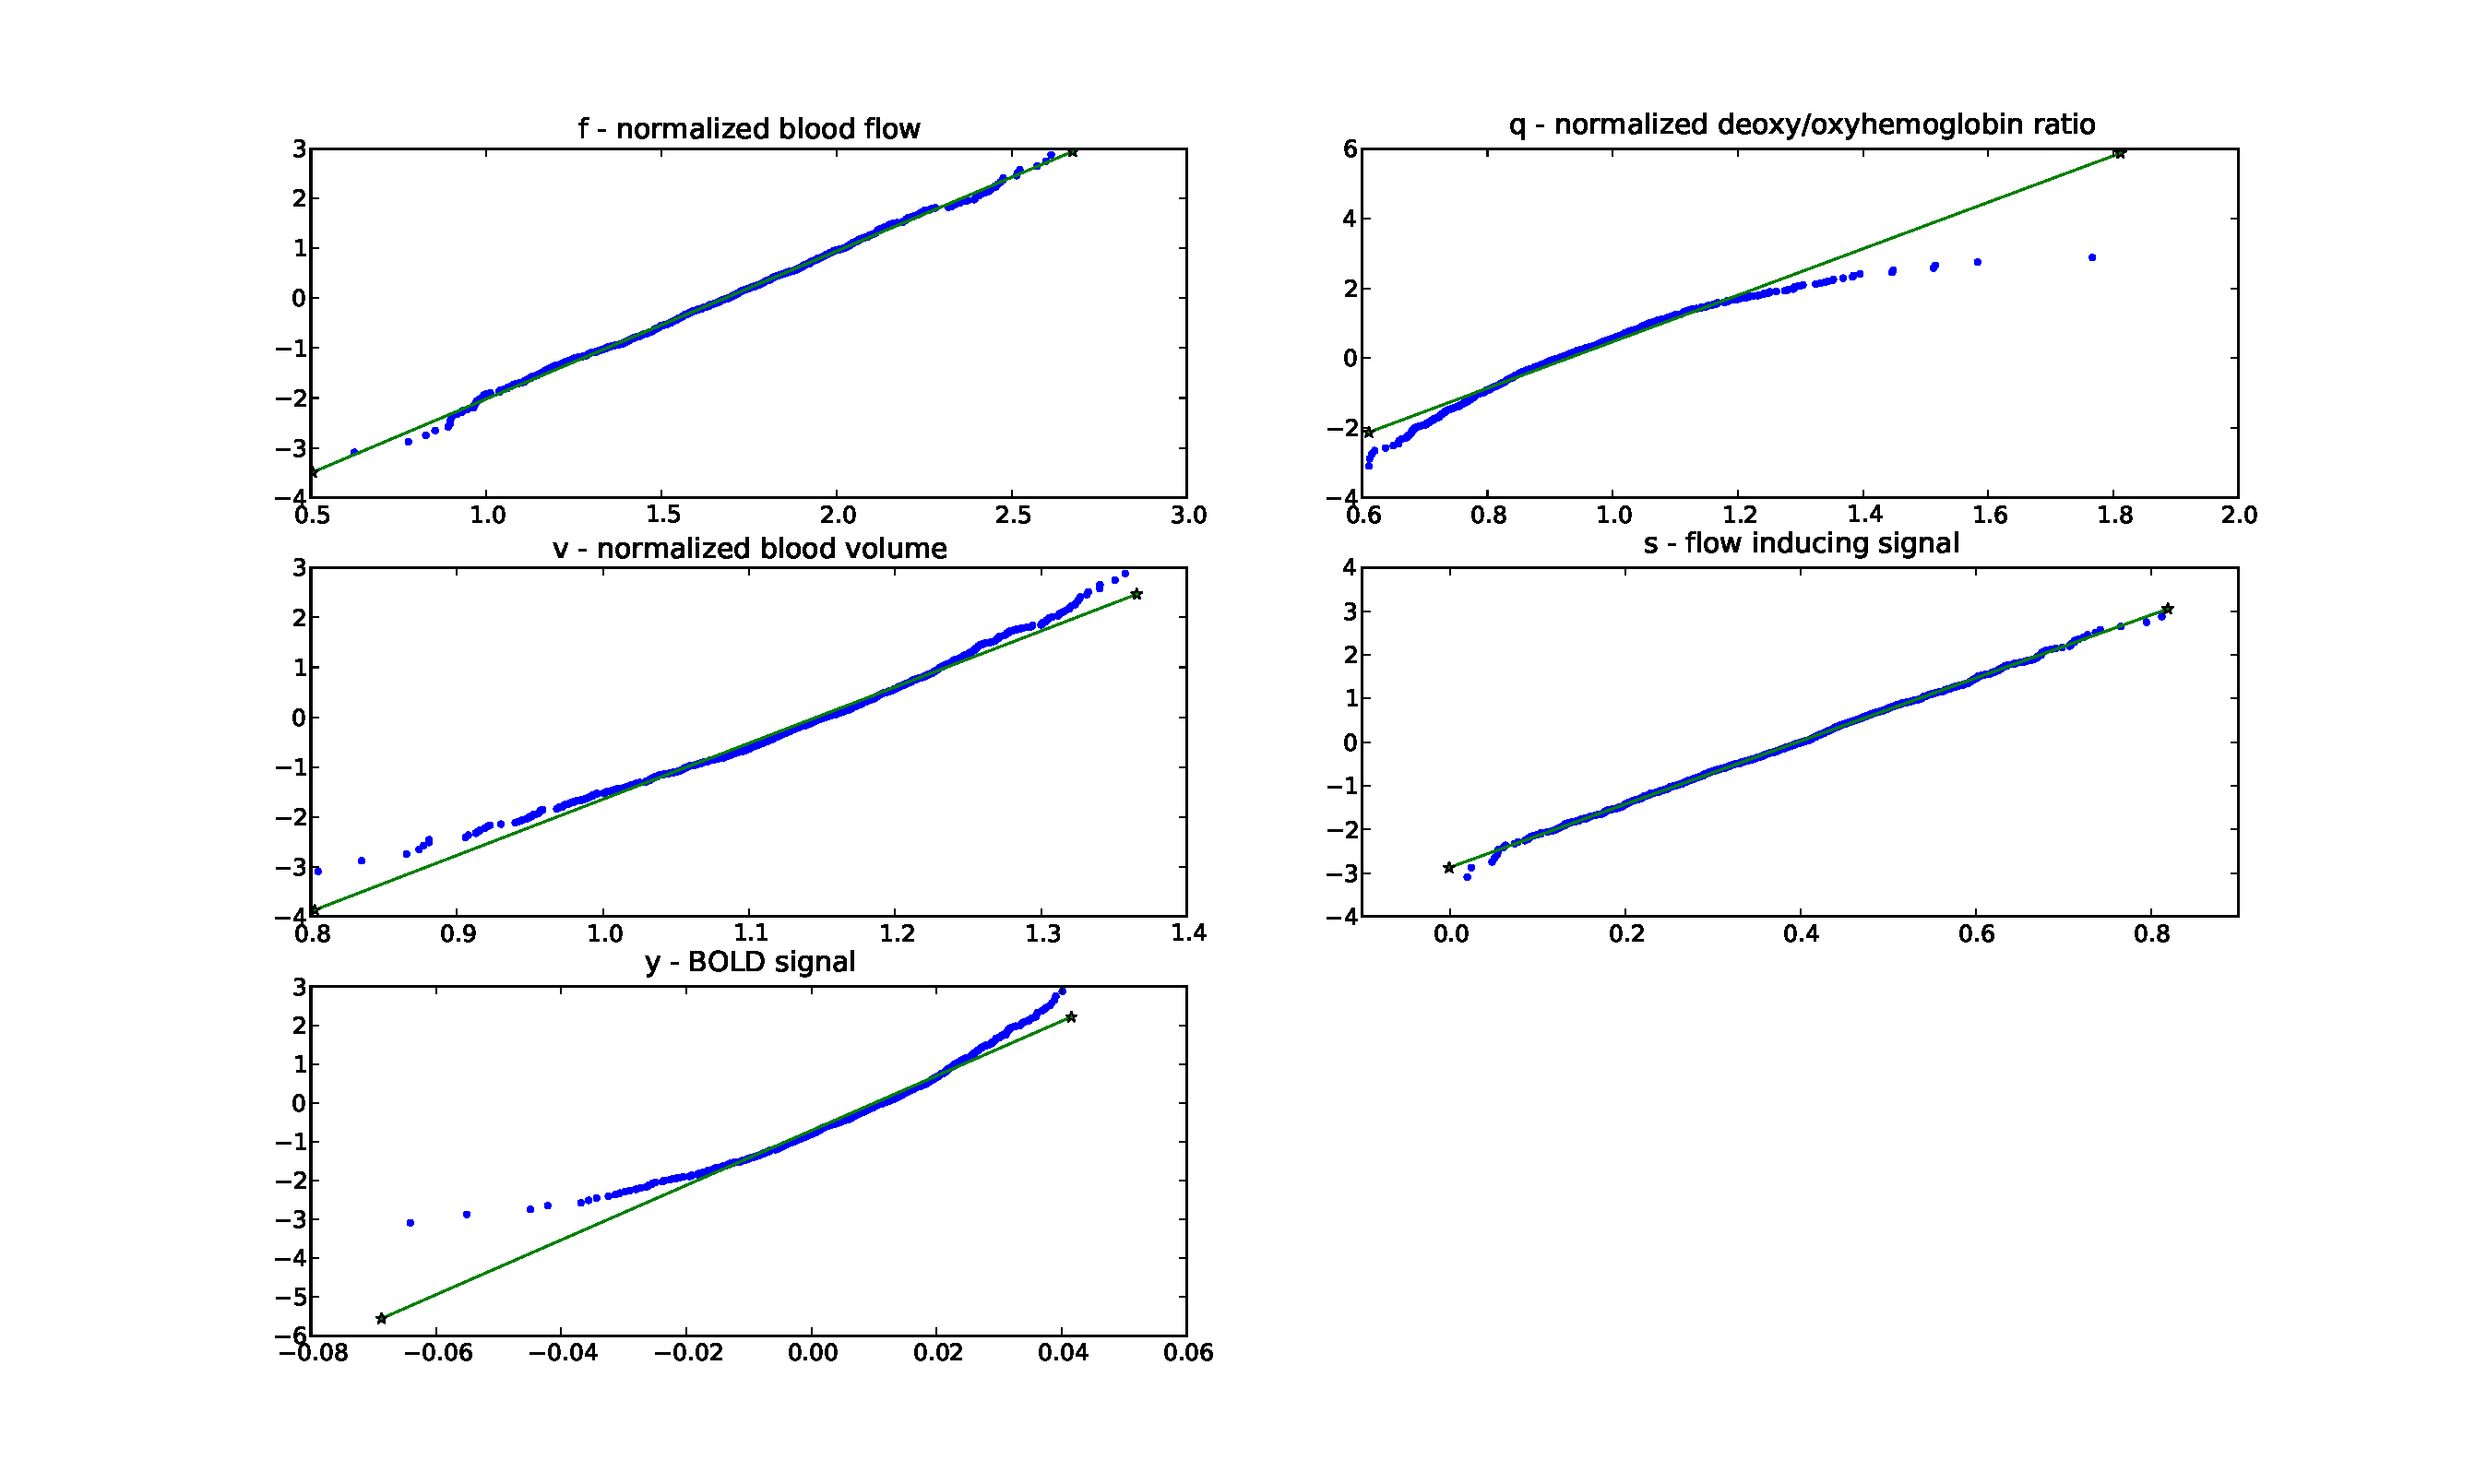
\includegraphics[trim=6cm .75cm 6cm .75cm,width=16cm]{images/gauss_step_1sec_3sigma.pdf}
\caption{Distributions of state variables after simulating for 1s}
\label{fig:trans1s}
\end{figure}

\section{Conclusion}
These other methods ....

\chapter{Particle Filters}
\section{Introduction}
Particle filters, a type of Sequential Monte Carlo (SMC) methods
are a powerful way of estimating the posterior probability distribution
of a set of parameters give a timeseries of measurements. Unlike Markov 
Chain Monte Carlo estimation, Sequential Monte-Carlo methods are designed
to be used with parameters that vary with time. Unlike variations of the
Kalman filter, particle filters do not make the assumption that noise
is Gaussian. Thus particle filters are often the best solution to bayesian 
tracking for non-linear, non-gaussian systems. 

\subsection{Model}
\label{sec:Particle Filter Model}
The idea of the particle
filter is to start with a wide mixture PDF of possible parameter sets, 
and then, as measurements come in, to weight more heavily parameter sets 
that tend to give good estimations of the measurements. The reliance on
an initial mixture PDF can introduce bias; however, this effect can be
minimized by alterring the initial weights in the mixture pdf. Of course
every gradient descent must choose starting points and it is often quite
easy to establish a reasonable range of parameters, especially when the
model being used has a physical meaning. Suppose a set or stream of measurements
are given, $\{y(t), t = 1, 2, 3, ... T\}$, where $T$ is permitted to go
 to infinity. Then the goal is to find the 
parameters, $\hat{\theta}$, and underlying state time series, $\hat{x}[0:T]$
that minimize the difference between $\hat{y}[0:T]$
and $y[0:T]$. In our case, we will assume that we know the form
of the model, which is based on first principals, and that
there is some true $\theta$ and a true time-series of underlying
state variable, $x[0:T]$ that drives $y[0:T]$. Assuming a model form 
such as we do here reduces model variance, potentially at the cost of increased
bias (or systematic) error. We will assume a basic state space model:

\begin{equation}
\dot{x}(t) = f(t, x(t), u(t), \theta, \nu_x)
\end{equation}

\begin{equation}
y(t) = g(t, x(t), u(t), \theta, \nu_y)
\end{equation}

Where $x(t)$ is a vector of state variables, $\theta$ is a vector of system
constants, $u(t)$ is a stimulus, $y(t)$ an observation, and
$\nu_x$ and $\nu_y$ are random variates. Obviously any one of these could
be a vector, so for instance $u(t)$ could encode multiple types of stimuli.

Although not strictly necessary for particle filters, we will make a few
assumptions based on the particular type of systems faced in biological 
processes. First, the systems are assumed to be time invariant. This 
assumption is based on the idea that if you froze the system for $\Delta t$
seconds, when unfrozen the system would continue as if nothing happend. 
Few biological systems are predictable enough for them to be summarized
by a time varying function. Even systems that one might assume work in that
way are actually much more complicated. The heart may seem like an obvious
exception, however, the period between heartbeats vary often enough that prediction
would necessitate another state-space model. In short, we
assume no parameters are time varying, because not enough information exists to
describe any of theme in that way. Luckily particle filters are capable 
of dealing with non-white, non-Gaussian noise, so unanticipated influence
may be re-factored as noise. Secondly we assume that input cannot directly
influence the output, which in the case of the BOLD signal is a good assumption.
%Third, through some sort of preprocessing, we will assume that $\nu_d$ can be
%decreased or completely removed, since it 
Third, we will assume noise is additive, and that $\nu_x$ may be projected into
a Weiner, or other summing process that is additive with $g$ and $\nu_y$, which
will be named $\nu_d$.
Finally, $x(t)$ will encapsulate $\theta$, the unknown model constants, which
means that the vector $\dot{x}$ will always have members
that are 0. The results of these assumptions are a simplified version of the
state space equations:

\begin{equation}
\dot{x}(t) = f(x(t), u(t))
\label{eq:stateass}
\end{equation}

\begin{equation}
y(t) = g(x(t)) + \nu_y + \nu_d
\label{eq:measass}
\end{equation}

Because $\nu_d$ is something akin to and additive Weiner process $y[0:T]$, it 
will include low frequency noise. $\nu_y$ on the other hand will cause i.i.d. noise
in $y[0:T]$. For some of the tests, I will use de-trending methods to reduce the effects of 
$\nu_d$, the remainder of which will be re-factored into $\nu_y$. Both $\nu_d$ and $\nu_y$
have biological and non-biological sources. MR can lead to both types of noise, 
as demonstrated in \cite{Smith1999}. Meanwhile changes in metabolism, heart rate, or
other biochemical intervention could all lead to either $\nu_d$ or $\nu_y$.

\subsection{Prior}

The goal of the particle filter is to evolve a probably distribution 
$Pr(\hat{x}(T) | u[0:T], y[0:T])$,
that asymptotically approaches the probability distribution $Pr(x(T) | u[0:T])$.
Considering that $y$ contains measurement noise as well as noise from $x$,
 it is clear that $Pr(x(t) | u[0:T])$ is not a single true value
but a true posterior. 
To begin with, the particle filter starts with a prior distribution, and $N_p$
particles need to be drawn from that distribution, $\alpha(x)$:
\begin{equation}
\{\hat{Pr}x_i(0),w_i] : x_i(0) \sim \alpha(x), w_i = \frac{1}{N_p}, i \in \{1, 2, ... , N_p\} \}
\end{equation}

Where $N_p$ is the number of particles or points used to describe the prior 
using a Mixture PDF. 
\begin{equation}
\hat{Pr}(x(0) = \hat{x}) = \sum_{i=1}^{N_p} w_i\delta(\hat{x} - x_i(0) ) dx
\end{equation}
Where $\delta(x-x_0)$ is 1 if and only if $x = x_0$ (the Kronecker delta function).

If a true prior is preferred, then the weights
should all be $1/N_p$, and since $x_i$ was drawn from the prior, this will
be an approximation of the prior distribution. If a relatively flat prior is 
preferred, then each particle's weight could be divided by the density, $\alpha(x_i)$,
which creates a flat prior with support points in the region of $\alpha(x)$. Either
way, $\alpha(x)$ should be much broader than the true posterior, $Pr(x(0))$, since the
choice of support points is crucial to the convergence of any sampling importance
algorithm. 
For the BOLD signal all the parameters have been studied and have relatively well
known mean and variance, so a prior could be very helpful. We ran simulations for
both normalized and un-normalized priors, although we believe in cases such as this,
where a good prior exists, it should be used. 
For strictly positive parameters (members of $x$) we used a gamma distribution,
whereas for parameters that could be negative, we used a Gaussian distribution. In
both cases standard deviations twice that found in previous studies were used.

Note that all the probabilities implicitly depend on $u[0:T]$, so those terms 
will be left off for simplicity.
Once the probability, $\hat{Pr}(x(T) | x[0:T-1], y[0:T-1])$ has been found
(initially this is just Mixture approximating the prior since no measurements are 
available and no previous probabilities are available), its possible to approximate
the probability for short times between times when measurement is available, by shifting
the probability according the progression of the state equations. This is only 
an approximate, since integrating $\nu_d$ should increase uncertainty as
time without a measurement passes. 

\begin{equation}
\hat{Pr}(x(T+\Delta t)) \approx 
\sum_{i=1}^{N_p} w_i\delta\left(x - (x_i(T) + \int_T^{T+\Delta} \dot{x}_i(t) dt) \right)
\end{equation}

\subsection{Weighting}
When a measurement becomes available it is incorporated into the probability.
This process of incorporating new data is called sequential importance sampling,
and eventually causes the probability to converge. The weight is defined
as

\begin{equation}
w_i(T) \propto \frac{\hat{Pr}(x_i[0:T] | y[0:T])}{q(x_i[0:T] | y[0:T])}
\label{eq:weightfunc}
\end{equation}

where $q$ is called an \emph{importance density}, meaning it decides where
the support points for $x(T)$ are located. To remove the bias due to the
location of the support points, we divide by $q(x_i[0:T] | y[0:T])$. By dividing by 
the posterior density of the support points (particles), the effect of the particle 
distribution may be removed from the posterior density. As a result the weight
is dependent solely based
on $\hat{Pr}(x_i[0:T] | y[0:T])$, the probability of the $i^{th}$ particle's measurements
being different from $y[0:T]$ due to noise alone.
An example of an importance density would be drawing a large
number of points from the standard normal, $N(0,1)$ and then weighting each point, $l$ by 
$1/\beta(l), \beta \sim N(0,1)$. Of course if there is a far off peak in
the posterior that $q$ does not allocate support points in, there will 
be a quantization error, and that part of the density can't be modeled. This is why
it is absolutely necessary that $q$ covers $\hat{Pr}(x_i[0:T] | y[0:T])$.

$q(x_i[0:T] | y[0:T])$ may be simplified by assuming that $y(T)$ doesn't contain 
any information about $x(T-1)$, which is more practical since knowledge of future
measurements is impractical. 

\begin{eqnarray}
q(x[0:T] | y[0:T]) & = & q(x(T) | x[0:T-1], y[0:T])q(x[0:T-1] | y[0:T]) \nonumber \\
& = & q(x(T) | x[0:T-1], y[0:T])q(x[0:T-1] | y[0:T-1]) \nonumber \\
& = & q(x(T) | x(T-1), y[0:T])q(x[0:T-1] | y[0:T-1])
\end{eqnarray}

In this paper we will use 
$q(x_i(T) | x_i(T-1), y[0:T]) =  \hat{Pr}(x_i(T) | x_i(T-1))$,
based on the Markov assumption, and the belief that the state space model is 
able to approximate the true state. This means that prior to re-weighting 
particles, the particles will be distributed the same as the previous time but
moved forward according to the integration of $f(x(t), u(t))$.

In addition to $q(x_i(T) | x_i[0:T-1], y[0:T])$, the weight is also based on $Pr(x_i[0:K] | y[0:K])$,
which may be broken up as follows.
\begin{eqnarray}
\hat{Pr}(x[0:T] | y[0:T]) & = & \frac{\hat{Pr}(y[0:T], x[0:T])}{\hat{Pr}(y[0:T])} \nonumber \\
 & = & \frac{\hat{Pr}(y(T), x[0:T] | y[0:T-1]) \cancel{\hat{Pr}(y[0:T-1])}}{\hat{Pr}(y(T) | y[0:T-1]) \cancel{\hat{Pr}(y[0:T-1])}} \nonumber \\
 & = & \frac{\hat{Pr}(y(T)| x[0:T], y[0:T-1]) \hat{Pr}(x[0:T] | y[0:T-1])}{\hat{Pr}(y(T) | y[0:T-1]) } \nonumber \\
 & = & \frac{\hat{Pr}(y(T)| x[0:T], y[0:T-1]) \hat{Pr}(x(T) | x[0:T-1], y[0:T-1]) \hat{Pr}(x[0:T-1] | y[0:T-1])}{\hat{Pr}(y(T) | y[0:T-1])} \nonumber \\
\end{eqnarray}

Using the assumption that $y(t)$ is fully constrained by $x(t)$ \autoref{eq:measass},
and that $x(t)$ is fully constrained by $x(t-1)$ \autoref{eq:stateass}, we are able to
make the reasonably good assumptions that:
\begin{equation}
\hat{Pr}(y(T) | x[0:T], y[0:T-1]) = \hat{Pr}(y(T) | x(T))
\end{equation}

\begin{equation}
\hat{Pr}(x(T) | x[0:T], y[0:T-1]) = \hat{Pr}(x(T) | x(T-1))
\end{equation}

Additionally, for the particle filter $y(T)$ and $y[0:T-1]$ are 
given, and therefore constant across all particles. Thus $\hat{Pr}(x[0:T] | y[0:T])$
may be simplified to:
\begin{eqnarray}
\hat{Pr}(x[0:T] | y[0:T]) & = & \frac{\hat{Pr}(y(T)| x[0:T], y[0:T-1]) \hat{Pr}(x(T) | x[0:T-1], y[0:T-1]) 
            \hat{Pr}(x[0:T-1] | y[0:T-1])}{\hat{Pr}(y(T) | y[0:T-1])} \nonumber \\
& = & \frac{\hat{Pr}(y(T)| x(T)) \hat{Pr}(x(T) | x(T-1)) \hat{Pr}(x[0:T-1] | y[0:T-1])}{\hat{Pr}(y(T) | y[0:T-1])} \nonumber \\
& \propto & \hat{Pr}(y(T)| x(T)) \hat{Pr}(x(T) | x(T-1)) \hat{Pr}(x[0:T-1] | y[0:T-1])
\end{eqnarray}

Plugging these simplifications into \autoref{eq:weightfunc} leads to:
\begin{eqnarray}
w_i(T) & \propto & \frac{\hat{Pr}(y(T)| x(T)) \cancel{\hat{Pr}(x(T) | x(T-1))} \hat{Pr}(x[0:T-1] | y[0:T-1])}
                         {\cancel{\hat{Pr}(x_i(T) | x_i(T-1))}q(x[0:T-1] | y[0:T-1])} \nonumber \\
& \propto & w_i(T-1)\hat{Pr}(y(T)| x(T)) 
\label{eq:weightevolve}
\end{eqnarray}

Thus, by making the following relatively weak assumptions, evolving a posterior
density  is easy and requires almost no knowledge of noise distribution.
\begin{enumerate}
\item $f(t, x(t), u(t)) = f(x(t), u(t))$ and $g(t, x(t), u(t)) = g(x(t))$ provide 
a sufficiently flexible model to encapsulate the true time series.
\item $E[\nu_d] = 0$ and $E[\nu_y] = 0$, and $\nu_x = d\nu_d$, $\nu_y$ are stationary
\item The PDF $q(x_i(0))$ (the prior) fully covers $Pr(x_i(0))$
\item Markov Assumption: $Pr(x(T) | x[0:T]) = Pr(x(T) | x(T-1))$
\item $q(x[0:T-1] | y[0:T]) = q(x[0:T-1] | y[0:T-1])$
\end{enumerate}

\subsection{Basic Particle Filter Algorithm}
From the definition of $w_i$, the algorithm sequential importance sampling (SIS) 
is relatively simple. 

\begin{algorithmic}
\STATE Initialize $N_p$ Particles: 
        $\{x_i(0),w_i(0) : x_i(0) \sim \alpha(x), w_i(0) = \frac{1}{N_p}, i \in \{1, 2, ... , N_p\} \}$
\STATE $T$ = \{Set of Measurement Times\}
\FOR{$t$ in $T$}
    \FOR{$i$ in $N_p$}
        \STATE $x_i(t) = x_i(t-1) + \int_{t-1}^t f(x(\tau), u(\tau)) d\tau $
        \STATE $w_i(t) = w_i(t-1)\hat{Pr}(y(t) | x(t))$
    \ENDFOR
\ENDFOR

\STATE At $t + \Delta t$, $t \in T$, $\hat{Pr}(x(t+\Delta t)) \approx 
\sum_{i=1}^{N_p} w_i(t)\delta\left(x - (x_i(t) + \int_t^{t+\Delta t} f(x(\tau), u(\tau)) d\tau) \right)$
\end{algorithmic}
The result is then a discrete approximation of the posterior distribution. 

\subsection{Resampling}
\label{sec:Particle Filter Resampling}
As a consequence 
of the wide prior distribution (required for a proper discretization of a continuous
distribution), there will be many particles with insignificant weights. While this does help
describe the tails of the distribution very well, it means that only a small portion of the
computation will be spent describing the most probable region. Ideally every particle would 
equally decrease the entropy of the distribution, thus the lower the variance of the weights,
the more efficiently the discrete distribution is in describing the continuous distribution. 
A common measure of "Particle Degeneracy" is the effective number of particles, described
in (Bergman "Navigation and Tracking Applications", 1999, J S Liu and R Chen "Sequential 
Monte Carlo Methods for Dynamical Systems", 1998), which is based on the "true weight"
of each particle. Of course the true weight is unknown, so a heuristic approximating 
$N_{eff}$ is used:
\begin{equation}
\hat{N}_{eff} \approx \frac{N_p}{\sum_{i=1}^{N_p} w_i^2}
\label{eq:neff}
\end{equation}
Any quick run of a particle filter will reveal that unless the prior is particularly accurate,
$N_{eff}$ drops precipitously.  To alleviate this problem
a common technique known as resampling must be applied. The idea of re-sampling is to 
draw from the approximate posterior, thus generating a replica of the posterior with 
a support more suited to the distribution. Thus, if weights are all set to $1/N_p$, and 
$N_p$ points are drawn from the posterior,
\begin{equation}
\hat{\chi}_j \sim \left(\sum_{i=1}^{N_p} w_i(t)\delta(x - x_i(t))\right), j \in \{1, ..., N_p\}
\end{equation}
then $\hat{\chi} \sim \hat{x}$ should hold. Unfortunately, this isn't necessarily the truth: since the support is
still limited to the original particles, the number of unique particles can only go down.
This effect, often dubbed "particle impoverishment" can result in excessive quantization
errors in the final distribution. However, there is a solution. Instead of sampling from the
discrete distribution, a smoothing kernel is applied, and $\hat{\chi}_j$ are drawn from
that distribution. Because the distribution is continuous, there is no way for a collapse
of the particles to occur. The question then, is how to decide on the smoothing kernel. 
Often times the easiest way to sample from the continous distribution is to break the 
re-sampling down into two steps. First a member of the discrete distribution is randomly
selected based on the weights, and then based on the smoothing a nearby state variable 
is selected. The process of the selection will be defined as:
\begin{equation}
\chi_i = x_i + h\sigma \epsilon
\end{equation}
Where $h$ is the bandwidth, $\sigma$ is the standard deviation such that $\sigma \sigma^T = cov(x)$
and $\epsilon$ is drawn from the chosen kernel.
It has been proven that when all the elements of the mixture
have the same weight, as is the case after basic resampling, the kernel that minimizes the 
MSE between the estimated and true posterior is the Epanechnikov Kernel (cite Improving Regularised
Particle Filters, C Musso, N Oudjane and F LeGrand). 
\begin{equation}
K = \left\{
\begin{array}{lr}
\frac{n_x+2}{2c_{n_x}}(1-\|x\|^2) & if\ \|x\| < 1\\
0 & otherwise
\end{array}\right.
\end{equation}
%<more here>

If the noise is assumed to be Gaussian then it is possible to further optimize. 
Thus we let $h$ be defines as:
\begin{eqnarray}
h = [N_s8c^{-1}_{n_x}(n_x + 4)(2\sqrt{\pi})^{n_x}]^{\frac{1}{n_x +4}}
\end{eqnarray}
and although it is very possible the underlying noise is non-gaussian, the Gaussian
may work, but sub-optimally. It has been proposed that (Monte Carlo Approximations for
General State-Space Models, markus Hurzeler and Hans R. Kunsch) if the underlying 
distribution is non-Gaussian, then using this bandwidth will oversmooth. 
In reality over smoothing
should not be too great an issue because the smoothing is only being applied to find new
particles. If the distribution is over smoothed then the algorithm may not converge as rapidly;
however, because the bandwidth is still based on particle variance, which will decay as 
particles are ruled out, it is still able to converge. In fact over smoothing is preferrable
to under smoothing, since the latter would result in false negatives, but the previous only
results in a slower decay of the variance. 
At the same time, as $n_x$, the number of dimensions in
$x$, goes to infinity, the standard deviation based approximation becomes less effective
(cite a Tutorial on Particle Filters for on-line non-linear non-gaussian bayesian
tracking, sanjeev arulampalam, simon maskell, neil gordon...).  Because of the high dimensionality of our system,
and limited measurements, it is helpful to have a broader bandwidth to explore the distribution. 
Nevertheless, because 
of the potentially wide smoothing factor applied by regularized resampling, performing this
step at every measurement would allow particles a great deal of mobility. This mobility is
the enemy of convergence, which is why regularized resampling should only be done when
$\hat{N}_{eff}$ drops very low (say less than 50). Other than the periodic regularized
resampling then, the regularized particle filter is nearly identical to the basic sampling
importance sampling filter (SIS). 

 \begin{algorithmic}
\STATE Initialize $N_p$ Particles: 
        $\{x_i(0),w_i(0) : x_i(0) \sim \alpha(x), w_i(0) = \frac{1}{N_p}, i \in \{1, 2, ... , N_p\} \}$
\STATE $T$ = \{Set of Measurement Times\}
\FOR{$t$ in $T$}
    \FOR{$i$ in $N_p$}
        \STATE $x_i(t) = x_i(t-1) + \int_{t-1}^t f(x(\tau), u(\tau)) d\tau $
        \STATE $w_i(t) = w_i(t-1)\hat{Pr}(y(t) | x(t))$
    \ENDFOR

    \STATE Calculate $N_{eff}$ with \autoref{eq:neff}
    \IF{$N_{eff} < N_R$ (recommend $N_R = min(50, .1N_p)$ )}
        \STATE Calculate empirical $\sigma$ 
        \STATE $h = [N_s8c^{-1}_{n_x}(n_x + 4)(2\sqrt{\pi})^{n_x}]^{\frac{1}{n_x +4}}$
        \STATE Redraw particles using (stratified) basic resampling
        \FOR{$i$ in $N_p$}
            \STATE Draw $\epsilon \sim K$
            \STATE $x_i = x_i + h \sigma \epsilon$
        \ENDFOR
    \ENDIF
\ENDFOR

\STATE At $t + \Delta t$, $t \in T$, $\hat{Pr}(x(t+\Delta t)) \approx 
\sum_{i=1}^{N_p} w_i(t)\delta\left(x - (x_i(t) + \int_t^{t+\Delta t} f(x(\tau), u(\tau)) d\tau) \right)$

 \end{algorithmic}

The ultimate effect of this regularized resampling is a convergence similar to simulated annealing
or a genetic algorithm. Versions of $x$ that are "fit" (give good measurements) spawn more children 
nearby which allow for more accurate estimation near points of high likelihood. 
As the variance of the estimated
$x$'s decrease, the radius in which children are spawned also decreases. Eventually the radius
will approach the width of the underlying uncertainty, $\nu_x$ and $\nu_y$.

\chapter{Proposed Approach}
\section{Goal}
The ultimate goal of this project is to provide a new set of tools
for analyzing FMRI data. Whereas SPM techniques have been highly 
successful at finding macroscopic regions of activation, linear 
modeling can carry significant bias error due to lack of model
flexibility. While adding parameters can significantly increase
error due to model variance, this effect is mitigated by the fact
that we plan to use a model that is based on first principals. The
purpose of this paper is thus to evaluate the potential of using
a particle filter along with the BOLD model to derive physical 
parameters. In so doing, we hope to be able to show that one or more
parameters are a suitable replacement for estimating voxel 
activation from a standard FMRI image. We also hope to show that 
estimated posterior distribution of the parameters, derived from
the particle filter, is able to provide an accurate measure of the
confidence interval.


\section{Choosing $\hat{Pr}(y(T) | x(T))$}
Choosing a representation of an unknown distribution is certainly tricky,
and so the fact that $\hat{Pr}(y(T) | x(T)) = \nu_d + \nu_y$ means that
there is a significant piece of the algorithm that is based primarily conjecture.
Studies of the noise in FMRI typically attribute noise to a Gaussian random
variable or an additive noise process with Gaussian steps. 

\subsection{Classical De-trending}
The non-stationary
aspect of a Weiner process as with $\nu_d$ is difficult to compensate for, and so various methods
have been developed to compensate for it. \cite{Tanabe2002} and \cite{Smith1999} have
demonstrated that this component is prevalent, and may in fact be a characteristic
of FMRI. In some studies, as many as half the voxels benefit from detrending, meaning
that this is certainly a serious barrier to inference. All the existing methods are performed
during the preprocessing stage, rather than as an integral part of analyzing the BOLD
signal. There is no shortage of theories on the "best" method of detrending, however
a head to head comparison, \cite{Tanabe2002}, showed that in most cases subtracting off
a spline works the best. The benefit of the spline versus wavelets, high pass 
filtering or other DC removal techniques is that the frequency response is not set.
A spline is able to move quickly when the signal is moving quickly, and move more
slowly when the signal moves more slowly. That said, the spline will still remove some
amount of signal, just like all of these methods. 

<image of de-spline'd lines with "true" lines>

\subsection{Delta Based Inference}
I also propose and test a different method of dealing with the so called "drift". 
Instead of comparing the direct output of the particle filter with the direct
measurement, the algorith compares the change in signal over a single TR. 
In most signal processing cases this would foolish, but that is because the 
general assumption that all noise is high frequency is not the case here.
In fact, every pipeline for the analysis of BOLD signal uses a high pass filter,
but low poss filters are rarely applied, because it is a well known fact that 
most of the signal is in the high frequency range and most of the noise is actually 
in the low frequency range. The particle filter is an 
extremely robust method of inference, and so I would assert that the particle
filter ought to be given as \emph{raw} data as possible. While taking direct measurements
without de-trending would give awful results, using the difference removes the 
DC component and turns a Weiner process into a Gaussian random variable. 

\begin{equation}
\Delta y = y(t) - y(t-1) = g(x(t)) - g(x(t-1)) + \nu_y(t) - \nu_y(t-1) + \nu_d(t) - \nu(t-1)
\label{eq:measass_delta}
\end{equation}

Because $\nu_d$ is a Weiner process, then $\nu_d(t) - \nu_d(t-1)$ is simply a Gaussian step. If
$\nu_d$ is some other additive process, the difference will still be one of a few stable
distributions. If $\nu_y$ is i.i.d. then the resulting distribution will still be zero mean
with a maximum variance of twice the original variance. All the assumptions made originally
for the particle filter hold, and all of the parameters may be distinguished based on
the step sizes, thus it is not unreasonable to attempt to match the string of step sizes
rather than string of direct readings. 

<frequency response graphs, highlighting noise frequency range and signal frequency range>

\subsection{Weighting Function}
Because $\hat{Pr}(y(T) | x(T))$, what I will call the weighting function,
is based on an unknown distribution, it is necessary to decide on a function
that will approximate $\hat{Pr}(y(t) | x(T))$. Obviously the function, $\omega(y(t), f(x(t))$
needs to be centered at zero and have a scale comparable to the signal levels.
Obviously if the actual noise present in $y(t)$ were to be known, then that would
be the best distribution for $\Omega$. In that case, particles that fell
far out on that distribution would be statistically impossible representations
of the system, and it would be completely reasonable to throw such particles away.
While a Gaussian function is the natural choice, because this distribution
and weight are unknown we wanted to try distributions
with wider tails, so that outliers don't completely destroy particle's weights
(and thus convergence proceeds more slowly).

Another natural choice might be one of the robust estimator weight functions, for
example the Huber or bi-square. For the purpose of this work we will stick
with long tailed distributions, however it is worth noting that long tails
may not be the optimal choice in all, or even this situation. The justification
for long tailed distributions is that we believe the noise to be long tailed,
and the variance of the noise is not well known.

Therefore, we tried three weighting functions based on three distributions: Gaussian, 
Laplace and the Cauchy. The standard deviation of the distribution is extremely
important to the convergence of particle filter. A standard deviation that is 
too large will not allow the distribution to converge in any reasonable number of 
measurements. A standard deviation below the standard deviation of the noise 
will cause the algorithm to throw out perfectly acceptable particles. 
The weighting function ultimately will shape the output distribution, $P[y]$, into that
distribution, however the distribution of $x$ will still approach a reasonable
estimate of its true distribution. Even an overly wide weighting function, will
allow the Gaussian Mixture estimate of $X$ to converge to the correct location 
parameters of the "real" posterior distribution, though the scale parameters may 
be overly large.

A reasonable method of setting the standard deviation of $\Omega$ may be by 
taking a small sample from "resting" data and using the sample standard deviation.
Since this is the first attempt at using particle filters for modeling the 
BOLD model, in this work we set the standard deviation manually at <weight standard dev>,
because it gives a more consistency and control. Of course this could be taken
further, by testing the sample data against a set of stock distributions
and choosing the best fit. This of course depends on having enough samples
to make a reasonable inference, which may not always exist. 

\section{Simple, Nonlinear Example}
A typical half wave rectifier takes a AC voltage circuit and removes
one half (say the negative half) of the signal. The resulting waveform
is still not DC, however it is then possible to use a capacitor to 
smooth the signal into something similar to DC, as shown in \autoref{fig:HalfWaveIO}.
There are other, more
complex circuits that convert the negative portion into positive and
waste less energy but but here we will keep the system simple.
Thus, let us consider a simple half wave rectifier circuit, shown in 
\autoref{fig:HalfWaveRectifier}.

The half wave rectifier circuit smoothes the gaps between high voltage
with a capacitor. Thus, when $u(t)G$ is less than $v_t$, the circuit will 
discharge the capacitor and maintain a non-zero voltage,
but when $u(t)G$ is greater than $v_t$, the output voltage will be set
by $u(t)G$ and the capacitor will charge up. We will assume a very simple
model for all the components, ignoring the complex nonlinear behavior
that can occur in a diode. 

\begin{figure}
\centering
\begin{circuitikz}[scale=2, american]
\draw
 (0,0)  node[transformer core] (T) {}
 (T.A1) -- (-1,0)
 (T.A2) -- (-1,-1.05)  to[V, v=$u(t)$] (-1, 0)
 (T.B1) -- (.5, 0) to[D, l=$v_t$] (1.5,0) to[C=$C$] (1.5, -1.05)
 (1.5, 0) -- (2.5, 0) to[R=$Rm$, v=$v_y$] (2.5, -1.05) -- (T.B2) 
 (T.base) node {G}
 (T.B1) to[open, *-*, v=$V_1$] (T.B2); 
\end{circuitikz}
\caption{An Example Half Wave Rectifier Circuit, where $G$ is the transformer
gain, $v_t$ is the activation voltage of the diode, $u(t)$ is the input at time $t$, 
$C$ is the capacitance, $R$ is the load resistance and $v_y$ is the output voltage}
\label{fig:HalfWaveRectifier}
\end{figure}

\begin{figure}
\centering
\caption{Example Input/Output of the Half Wave Rectifier}
\label{fig:HalfWaveIO}
\end{figure}

Although rectifiers are typically thought
of as receiving an AC circuit 60 Hz, we will ignore such specifics and 
assume the voltage across the output of the transformer is simply a scalar
multiple of the input voltage.  As discussed in the \autoref{sec:Particle Filter Model}
any variable with uncertainty must be part of the state variable. Therefore
the state variable will be: $X(t) = \{G, v_t, C, R_m, v_y\}$. Of course,
$u(t)$ cannot be allowed to be a square wave in such a system, since that
such a signal would never get across the transformer and regardless it
would necessitate an unrealistic infinite current across the capacitor.
The state equations would then be 

\begin{equation}
v_y(t)  = f(v_y(t-1, u(t)) =  \begin{cases} 
        u(t)G & \text{ if }  u(t)G-v_y \ge v_t\\
        v_y(t-1)\left(1 - \frac{\delta t}{R_mC}\right) & \text{ if }  u(t)G-v_y < v_t
    \end{cases} 
\end{equation}

To run the particle filter is relatively easy then, since there exists 
a recursive definition of the dynamic state variable, $v_y$. To start
with, an initial distribution must be assumed and while at first a 
Gaussian seems like a good idea, all the static state variables are strictly
positive and thus not well suited to the Gaussian. In this case then,
it would be wise to start with a Gamma distribution, and just be wary of
any standard deviation that gets larger than the prior mean. We will define
the gamma distribution as follows:

\begin{equation}
X \sim Gamma(k, \theta) \rightarrow f(x) = x^{k-1}\frac{e^{-x/\theta}}{\theta^k\Gamma(k)}
\end{equation}

where $\Gamma$ is the gamma function.
The in some ways the margin for error is decided by the weighting function, which
here will define as $W(V_y, v_{yi})$, where $V_y$ is the actual measurement, $v_y$ is the 
estimate based on all the particles, and 
$v_{yi}$ is the estimate by a particular (i$^{\text{th}}$) particle. The choice of this function is difficult,
and although the Gaussian is typically used, we found the exponential helpful
in dealing with particle deprivation.  The algorithm will then look like the following,

\begin{algorithmic}
\STATE Initialize $N_p$ Particles:
\FOR{$i$ in $N_p$}
    \STATE $G \sim Gamma(\frac{\mu^2_G}{\sigma^2_G}, \frac{\sigma^2_G}{\mu_G})$
    \STATE $v_t \sim Gamma(\frac{\mu^2_{v_t}}{\sigma^2_{v_t}}, \frac{\sigma^2_{v_t}}{\mu_{v_t}})$
    \STATE $C \sim Gamma(\frac{\mu^2_C}{\sigma^2_C}, \frac{\sigma^2_C}{\mu_C})$
    \STATE $R_m \sim Gamma(\frac{\mu^2_R}{\sigma^2_R}, \frac{\sigma^2_R}{\mu_R})$
    \STATE $v_y = 0$, (Assume the system has been off for a long time)
    \STATE let $X_i(0) = \{G, v_t, C, R_m, v_y\}$
    \STATE let $w_i(0) = 1$ or to make a flat prior, $w_i(0) = \frac{1}{Pr(X_i(0))}$ 
\ENDFOR
\STATE Run the Filter:
\FOR{$t$ in Set of Measurement Times}
    \FOR{$i$ in $N_p$}
        \STATE $v_{yi}(t) = f(v_{yi}(t-1), u(t))$
        \STATE (All other members of $X_i(t)$ remain the same)
        \STATE $w_i(t) = w_i(t-1)W(V_y(t), v_y(t))$
    \ENDFOR
\ENDFOR
\end{algorithmic}

Initially the particles will have the same output, $0$, however, as $u(t)$
changes, the response of each particle to that input will result in different
outputs. Particles that have a $v_{yi}$ near $V_y$ will be weighted higher,
and others farther away will be weighted lower. As the particle filter
runs, weights will compound resulting in a distribution that asymptotically
approaches the true joint distribution of the $X(t)$.  Of course, as we
mentioned in \autoref{sec:Particle Filter Resampling}, particles weighted zero do not significantly
contribute to the empirical distribution, so re-sampling may be necessary.

\chapter{Methods}
This paper describes two types of experiments; first we will cover
simulations which have the benefit of a ground truth, then we will
cover the methods used in the use of the particle filter on real data.

\section{Preprocessing}
\label{sec:Methods Preprocessing}
As discussed in the section on de-trending, the normal pipeline for analyzing
FMRI involves a great deal of preprocessing. In this paper we make an effort to
minimize any type of preprocessing that will degrade the signal. 
After FMRI data has been acquired it is always necessary to modify the
data in some way to make different runs comparable. Because FMRI signal
levels are unit-less, at the very least it is necessary to convert
the data into \% difference from the baseline. This process removes no data
from signal since it merely subtracting then dividing by a constant. This
is the signal that was input into the delta based particle filter.
Of course there are much more advanced ways of performing this task.
The generally accepted standard is actually to use a high pass filter, although the
cutoff frequency is application dependent and often applied haphazardly.
The high pass filter thus removes the DC component of the signal, and 
some amount of the so called "drift". The problem with this method is that it is
not adaptive to the input. Huge variations in drift frequencies can exist 
in a single time-series. Thus, a single cutoff frequency could miss a significant
drift component, or it could remove \emph{actual} signal, if the cutoff frequency is
set too high. This is why, as I mentioned in the De-trending section, a spline
based detrending method will generally give better results. 

For simulated and real images (tests with multiple time-series), tests were 
also run with and without Gaussian filtering with sigma of %not sure todo
were run, since it is standard
practice to apply a Gaussian spatial filter to the images at each timestep. Obviously
a spatial filter such as Gaussian filtering increased SNR but can also lead to less
precision in the output maps.

\section{Simulation}
We performed two types of simulations. First, we simulated a single BOLD time-series based
on a random chosen set of model parameters. This process was relatively straight forward
given the state-space equations for the BOLD signal. After a "true" signal was generated,
we then added a carrier level, since BOLD is typically measured as a \% difference from the
base level. Finally, we added Gaussian noise, and a Weiner Process to the clean signal. The
variance of the Gaussian noise may be expressed in terms of the desired noise SNR, $R$ as:
\begin{equation}
var(y_{noisy}) = var(y) / R
\end{equation}
Since SNR doesn't have quite the same meaning for a Wiener process based noise, the variance 
of the Gaussian steps was set to be:
\begin{equation}
var(y_{noisy}) = var(y) / (4R)
\end{equation}
Once this noisy simulated time series was generated, the exact same particle filter algorithm
that would later be run on full sized images, was run on this single voxel image. We ran
a series of tests to determine the convergence rate of the particle filter, the number
of particles that were required, how weighting functions compared, how different de-trending
methods compared with each other and, finally the variance of the result. By running the exact
time-series with different noise realizations, it was possible to determine the model variance.
As the reader may know, the error of an estimator may be calculated as:
\begin{equation}
MSE(\Theta) = Var(\Theta) + Bias(\Theta)^2
\end{equation}
The variance is an expression of how much the result would change for different noise realizations,
whereas the bias is an expression of how well the model matches the true underlying model. In
this case, because the same model is being used in the particle filter and underlying simulation,
the bias is actually zero. Obviously when this is calculated using \emph{real} data with an unknown
underlying state space equation, there will be some amount of bias error, but assuming that the
noise is similar to the noise used in these tests, the model variance will actually be about the
same. Thus calculating the model variance is extremely helpful in calculating how well determined
our model is, and how consistent it will be for real data. A single timeseries, as opposed to the
thousands present in a real image, makes it easier to 
compare the output with the ground truth, with various parameters. 

Second we used a modified version of the FSL tool 
POSSUM to generate an entire FMRI image from a parameter map. The parameter map was generated
by creating a random image, smoothing it with a large Gaussian kernel, then thresholding
the results. Finally connected regions were each given a set of parameters from a finite
list of randomly chosen parameter sets. The result was a four dimensional (length x width
x height x parameter) image with spatially varying parameters. Time-series of activation level
was generated for each set of parameters, then activation levels were fed into POSSUM's 
function for generating frequency domain data. The patche for POSSUM will be made available.
For each time-series in the simulate FMRI image, the final \emph{static} parameters are saved
into a parameter map. This parameter map may then be compared to the map used to generate the 
simulated data; additionally a new simulation using the calculated parameters may also be 
generated to test the functional difference between the two maps. This would give an absolute 
quantitative difference between the two parameter sets irrespective to parameter slopiness.
So for instance, if $V_0$ is halved, $\epsilon$ doubling may very well give a similar result.
In this case the \% difference between the parameters will be large in each case, but the functional
difference between the parameters will not be great. This is obviously a bad situation, which
is why we wanted to test for it.

\section{Real Data}
Finally, we also performed inference based on real FMRI data. The scanner we used...
%... more specifics...

The final result from calculating parameters with the real data was similar to that
from the results from the POSSUM simulated data. The difference being that there was
no ground truth the check it with. 

\chapter{Results}
\section{Single Time-Series Simulation}

Graphs: 

For simulated data, single timeseries:

For \{delta, DC/Spline\}, \{exponential, gaussian, cauchy\}, \{biased, unbiased initial\},
\{100, 500, 1000\} particles
\begin{enumerate}
\item Ground truth vs. Estimated signal during particle filter run
\item Ground truth vs. Estimated signal with final parameter set
\item True Parameters vs. Final Parameter Sets
\item Variance of final parameters when faced with same ground truth, different noise
\item MSE of (a new timeseries based on X(t) vs. ground truth) for all t
\item Estimator Variance based on different noise runs
\item Final Particle Distribution
\end{enumerate}

For Simulated Data, Full Volume:

%note to self, epsilon should probably be uniform between 0 and something
\section{Simulated Volume}
\begin{enumerate}
\item Parameter Map 
\item Error map of parameters
\item Histogram of \%errors between parameters
\item Activation Map based on a single region with high $\epsilon$, compared with linear
\end{enumerate}

\section{FMRI Data}
....

image comparing epsilon-map with GLM activation map

\chapter{Conclusion}

\bibliographystyle{apalike}
%\bibliographystyle{abbrvnat}
%\bibliographystyle{abbrv}
\bibliography{library}


\end{document}

%trash
%stream of new developments in modeling the BOLD signal, nothing has have been
%a plethora of new studies pushing advancements 
%the choice of analysis tools is still relatively limited. Every widely
%available analysis tool is based on parametric modeling, which requires
%prior knowledge of the noise distribution. Indeed, the linear methods
%usually applied are known not to be robust to non-gaussian, non-white
%noise, which is why so many pre-processing steps are necessary.
%These limitations cast a long shadow over any experiment that claims to be
%able to reject the null hypothesis, no matter the P-value. While obviously
%there is a correlation between the BOLD signal and actual activity, its
%possible the current parametric tests are over-estimating the actual amount
%of activity. Its also possible that the current methods underestimate
%actual activity. In this paper we propose a robust model-based approach to 
%activation detection that makes no assumptions about the underlying noise
%model.

